\documentclass{beamer}

\begin{document}
\huge
\begin{frame}{Eksempel 1}
	\huge
	Lag reknestykket
	\huge
	\[ \frac{1}{5}+\frac{3}{5} \]
\end{frame}	

\begin{frame}{Eksempel 1}
\begin{center}
	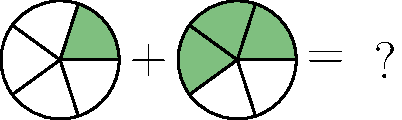
\includegraphics{fig1a}
\end{center}
\end{frame}

\begin{frame}{Eksempel 1}
	\begin{center}
		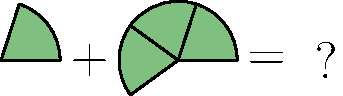
\includegraphics{fig1b}
	\end{center}
\end{frame}

\begin{frame}{Eksempel 1}
	\begin{center}
		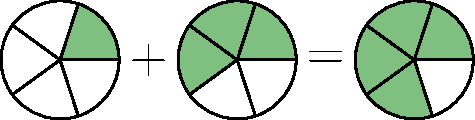
\includegraphics{fig1a2}
	\end{center}
\[ \frac{1}{5}+\frac{3}{5}=\frac{4}{5} \]
\end{frame}

\begin{frame}{Eksempel 2}

	Lag reknestykket
	
	\[ \frac{3}{7}+\frac{2}{7} \]
\end{frame}	

\begin{frame}{Eksempel 2}
	\begin{center}
		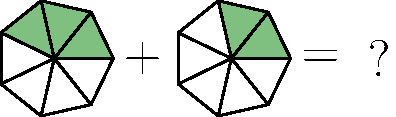
\includegraphics{fig2a}
	\end{center}
\end{frame}

\begin{frame}{Eksempel 2}
	\begin{center}
		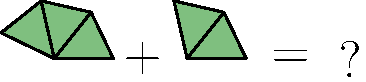
\includegraphics{fig2b}
	\end{center}
\end{frame}

\begin{frame}{Eksempel 2}
	\begin{center}
		
\includegraphics{fig2a2}
	\end{center}
\[ \frac{3}{7}+\frac{2}{7}=\frac{5}{7} \]
\end{frame}
\end{document}